\chapter{Model Development, Evaluation, and Serving}
\label{chap:model}

\section{Artifact identity and terminology}

The project evaluates four model states: Historical V2 (LightGBM), Serving Default V2 (Configured champion), and Current Candidate (CatBoost Balanced, status: \texttt{not\_promoted}) (Table~\ref{tab:model-identifiers}).

\begin{table}[H]
\centering
\caption{Model identifiers and runtime roles}
\label{tab:model-identifiers}
\begin{tabular}{llll}
\toprule
\textbf{Identifier} & \textbf{Model} & \textbf{Role} & \textbf{Status}\\
\midrule
Historical V2 & LightGBM & Historical artifact & Historical\\
Serving default \texttt{v2} & LightGBM & Configured champion & Unchanged\\
Current candidate & CatBoost balanced & Challenger & Not promoted\\
\bottomrule
\end{tabular}
\end{table}

\section{Model-development protocol}

Architecture operates via \textbf{distributed Spark data preparation with single-node Python estimator training}. Figure~\ref{fig:final-training-lifecycle} illustrates the end-to-end training lifecycle.

\begin{figure}[H]
\centering
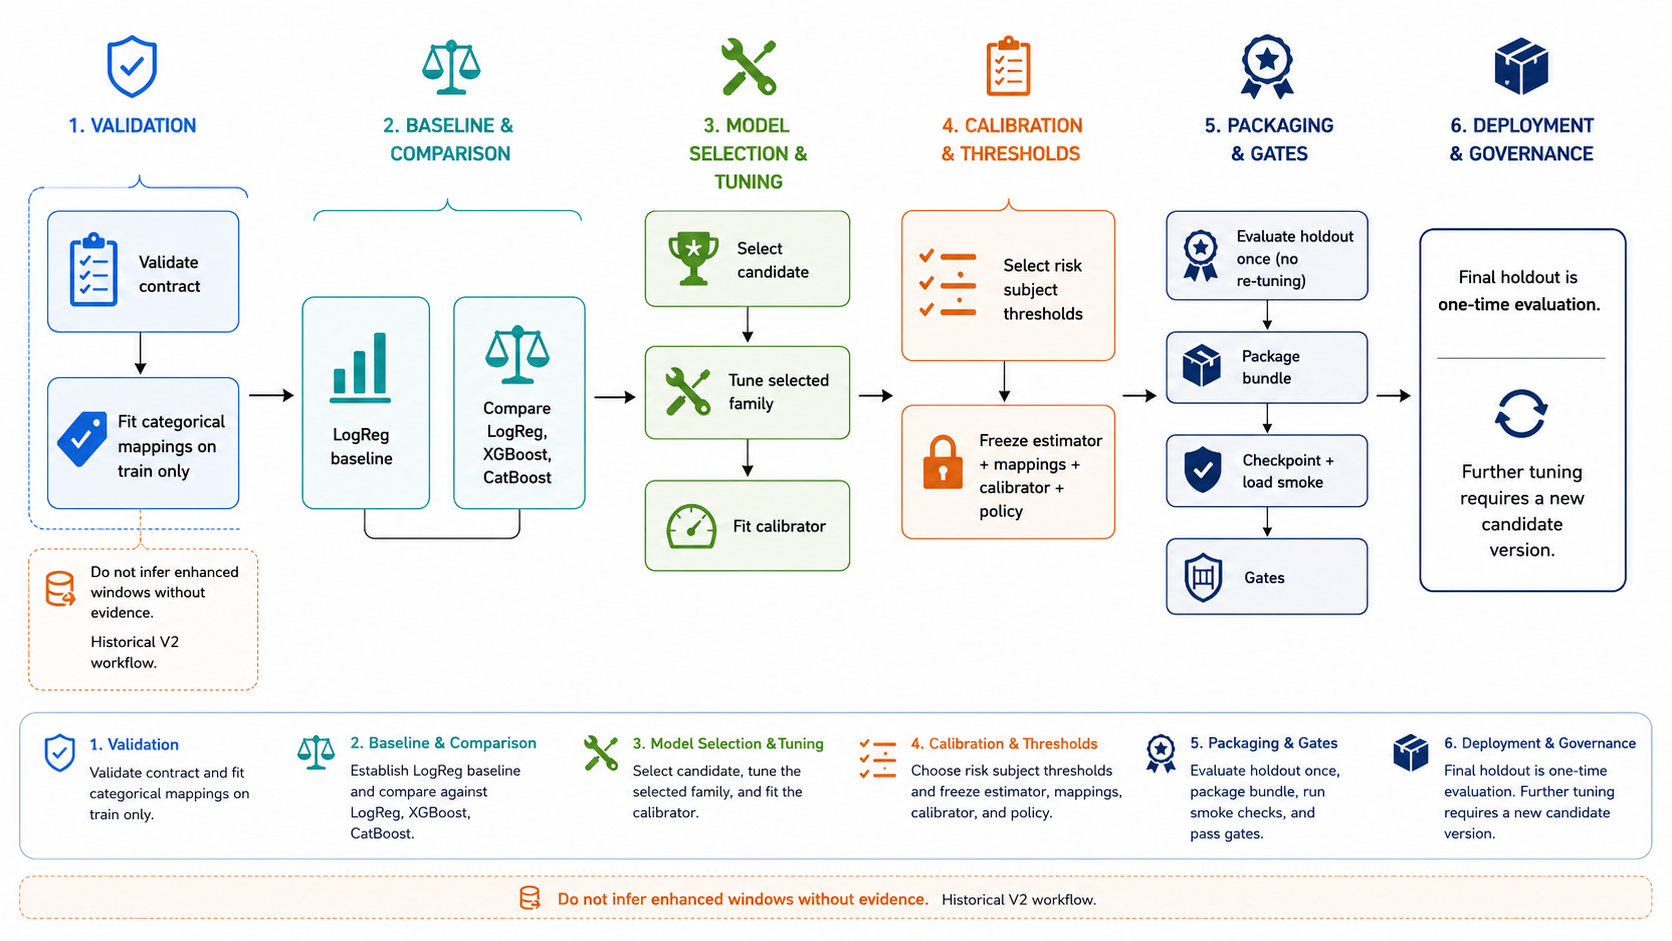
\includegraphics[width=\textwidth,height=0.36\textheight,keepaspectratio]{../../docs/diagrams/final/End-to-End-Model-Training-Lifecycle.png}
\caption[Model training lifecycle]{Model training lifecycle. Spark provides distributed data preparation; estimator fitting is single-node Python training.}
\label{fig:final-training-lifecycle}
\end{figure}


\section{PySpark MLlib DecisionTree baseline}

To satisfy BDA501 big-data ML baseline requirements, a PySpark MLlib \texttt{DecisionTreeClassifier} pipeline evaluates the \val{68}-feature vector across three dataset variants (Table~\ref{tab:mllib-decision-tree}).

\begin{table}[H]
\centering
\small
\rowcolors{2}{ReportGray!25}{white}
\caption{PySpark MLlib DecisionTree Baseline Performance}
\label{tab:mllib-decision-tree}
\begin{tabular}{llrrrrr}
\toprule
\textbf{Model variant} & \textbf{Split} & \textbf{PR-AUC} & \textbf{ROC-AUC} & \textbf{Precision} & \textbf{Recall} & \textbf{Time (s)}\\
\midrule
\texttt{baseline\_tree} & Validation & \val{0.0205} & \val{0.2329} & \val{0.6928} & \val{0.1574} & \val{13.5}\\
\texttt{baseline\_tree} & Holdout & \val{0.0209} & \val{0.2366} & \val{0.6641} & \val{0.1948} & \val{13.5}\\
\texttt{weighted\_tree} & Validation & \val{0.2666} & \val{0.6866} & \val{0.1564} & \val{0.6400} & \val{12.1}\\
\texttt{weighted\_tree} & Holdout & \val{0.2773} & \val{0.6984} & \val{0.1494} & \val{0.6583} & \val{12.1}\\
\texttt{undersampled\_tree} & Validation & \val{0.0284} & \val{0.4265} & \val{0.2791} & \val{0.5217} & \val{5.7}\\
\texttt{undersampled\_tree} & Holdout & \val{0.0278} & \val{0.4163} & \val{0.2039} & \val{0.5076} & \val{5.7}\\
\bottomrule
\end{tabular}
\end{table}

\section{Candidate models and selection}

Evaluation compares Logistic Regression, LightGBM, XGBoost, and CatBoost (Table~\ref{tab:model-family-comparison}). CatBoost Balanced achieved highest PR-AUC.

\begin{table}[H]
\centering
\small
\rowcolors{2}{ReportGray!25}{white}
\caption{Current model-family selection evidence}
\label{tab:model-family-comparison}
\begin{tabular}{llrrl}
\toprule
\textbf{Model} & \textbf{Training variant} & \textbf{ROC-AUC} & \textbf{PR-AUC} & \textbf{Decision}\\
\midrule
Logistic Regression & Weighted & \val{0.8219} & \val{0.3090} & Baseline\\
LightGBM & Weighted & \val{0.9116} & \val{0.5682} & Compared\\
XGBoost & Weighted & \val{0.8879} & \val{0.5529} & Compared\\
CatBoost & Weighted & \val{0.8757} & \val{0.5245} & Compared\\
CatBoost & Balanced & \val{0.9070} & \val{0.5703} & Selected\\
\bottomrule
\end{tabular}
\end{table}

\section{Current CatBoost candidate results}

Table~\ref{tab:official-v2-metrics} records candidate performance across validation and holdout splits.

\begin{table}[H]
\centering
\small
\rowcolors{2}{ReportGray!25}{white}
\caption{Current CatBoost candidate validation and holdout metrics}
\label{tab:official-v2-metrics}
\begin{tabular}{lrrrrrr}
\toprule
\textbf{Window} & \textbf{Threshold} & \textbf{PR-AUC} & \textbf{ROC-AUC} & \textbf{Precision} & \textbf{Recall} & \textbf{Brier}\\
\midrule
Validation selection & \val{0.50} & \val{0.5806} & \val{0.9081} & \val{0.3970} & \val{0.6220} & --\\
Holdout & \val{0.16} & \val{0.4266} & \val{0.8781} & \val{0.3820} & \val{0.5182} & \val{0.0248}\\
\bottomrule
\end{tabular}
\end{table}

\section{Packaging, checksum, and promotion}

The candidate promotion gate evaluated \val{9} criteria (Table~\ref{tab:v2-gates}). Due to holdout PR-AUC degradation (\val{0.4266} vs target \val{0.4582}), the promotion decision remains \texttt{not\_promoted}.

\begin{table}[H]
\centering
\small
\rowcolors{2}{ReportGray!25}{white}
\caption{Current candidate promotion gate}
\label{tab:v2-gates}
\begin{tabular}{lcc}
\toprule
\textbf{Gate} & \textbf{Result} & \textbf{Evidence}\\
\midrule
Holdout PR-AUC $\geq$ 0.4582 & Fail & \val{0.4266}\\
Holdout ROC-AUC $\geq$ 0.8746 & Pass & \val{0.8781}\\
Review precision $\geq$ 0.30 & Pass & \val{0.3820}\\
Calibration non-regression & Pass & Brier decreased\\
Artifact checksum & Pass & SHA-256 match\\
Artifact-load smoke & Pass & Manifest verified\\
Data contract verification & Pass & \val{94} checks ready\\
Version match & Pass & \texttt{v2}\\
Git clean & Fail & \texttt{git\_dirty=true}\\
\bottomrule
\end{tabular}
\end{table}

\begin{figure}[H]
\centering
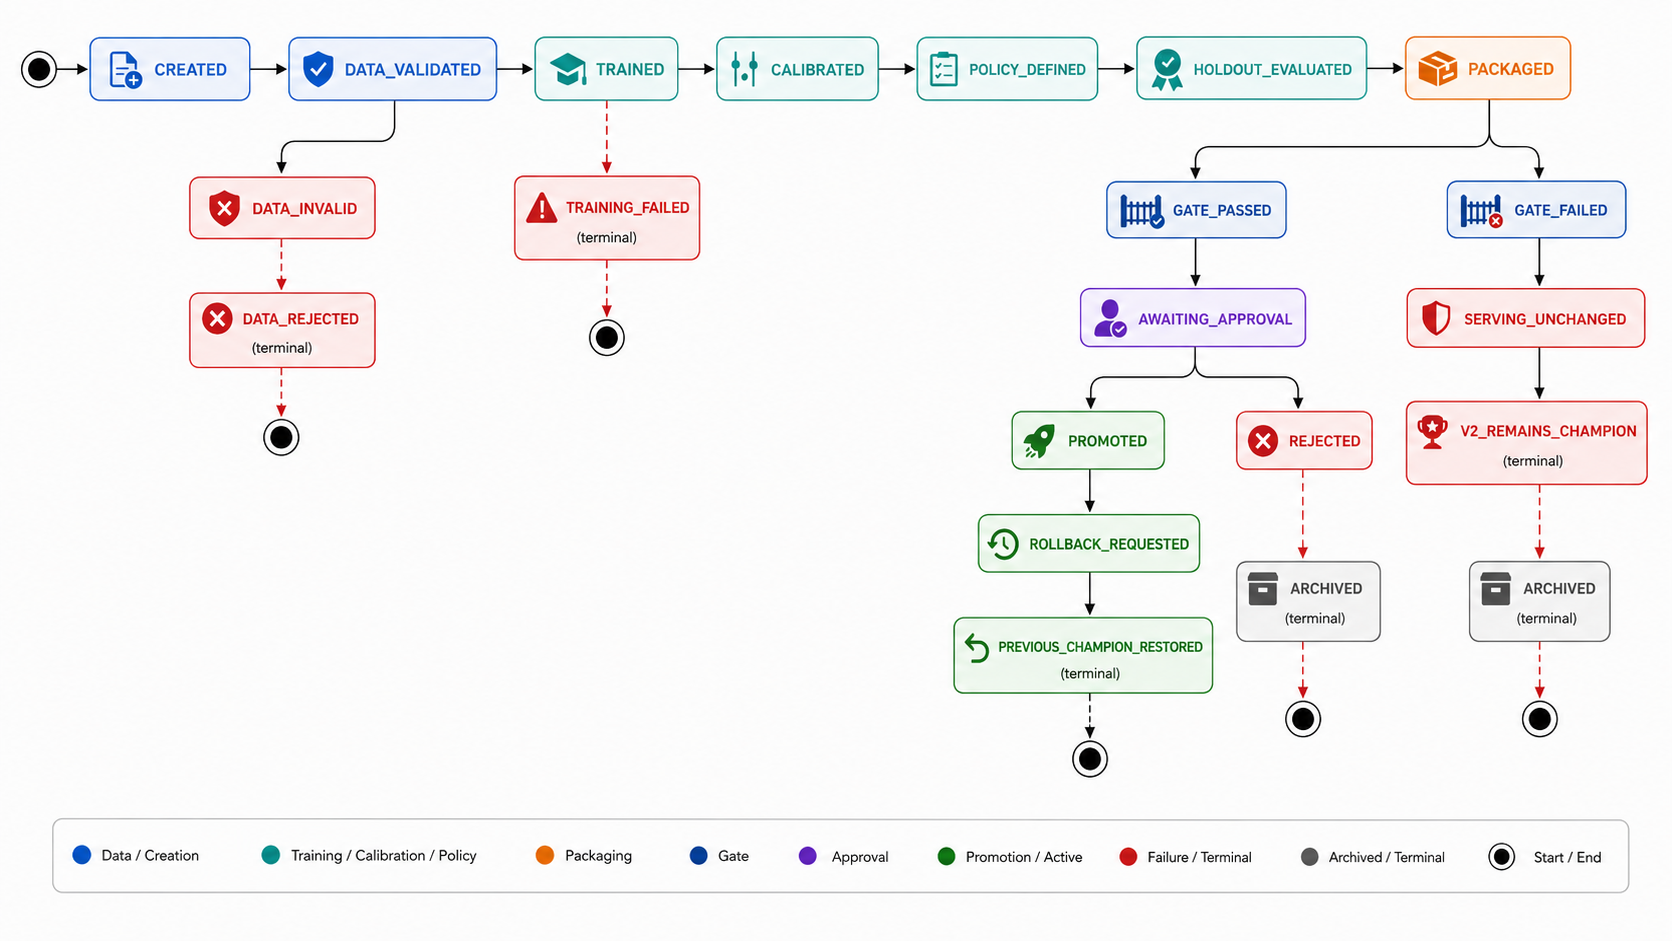
\includegraphics[width=\textwidth,height=0.48\textheight,keepaspectratio]{../../docs/diagrams/final/promotion-state-machine.png}
\caption[Promotion state machine]{Promotion state machine.}
\label{fig:final-promotion-state}
\end{figure}


\section{Request-time scoring}

Real-time scoring maps categoricals via persisted indexers, applies isotonic calibration, and computes TreeSHAP feature attributions \parencite{lundberg2017shap}. Responses support \texttt{full\_feature} and \texttt{partial\_demo} modes.
